\documentclass[a4paper]{article}
\usepackage[portuguese]{babel}
\usepackage[utf8]{inputenc}
\usepackage{indentfirst}
\usepackage{graphicx}
\usepackage{verbatim}
\usepackage{indentfirst}
\usepackage{setspace}
\usepackage[export]{adjustbox}
\usepackage{makeidx}
\usepackage{float}
\usepackage{pdfpages}
\usepackage{hyperref}
\usepackage{xcolor,listings}
\usepackage{textcomp}
\usepackage[width=160mm,height=220mm]{geometry}
\usepackage{mathtools}
\usepackage{lipsum}
\newcounter{question}
\setcounter{question}{0}
\usepackage{multicol}
\usepackage{wrapfig}
\usepackage{listings}
\usepackage{setspace}


\title{BDAD-Relatorio2}
\author{luistelmocosta }
\date{April 2016}
\onehalfspacing
\begin{document}


\title{\Huge\textbf{EasyPilot}\linebreak\linebreak
  \Large\textbf{Relatório 1}\linebreak\linebreak
  \linebreak\linebreak
  
\includegraphics[scale=0.1]{feup-logo.png}\linebreak\linebreak
  \linebreak
  \Large{Mestrado Integrado em Engenharia Informática e Computação} \linebreak\linebreak
  \Large{CONCEPÇÃO E ANÁLISE DE ALGORITMOS}\linebreak
  }
  
  \author{\textbf{2MIEIC05, E, 1}\\
  Luís Costa -  200806068\\
  Alexandre Ribeiro - up201205024\\
  José Mendes - up201200647\\
  \footnote{Github - \url{https://github.com/01alex/FEUP-CAL}}
  \linebreak\linebreak \\
  \\ Faculdade de Engenharia da Universidade do Porto \\ Rua Roberto Frias, s\/n, 4200-465 Porto, Portugal \linebreak\linebreak\linebreak
  \linebreak\linebreak\vspace{1cm}}
  
  \maketitle

\thispagestyle{empty}

\newpage

\tableofcontents

\newpage

\setcounter{secnumdepth}{0}
\section{INTRODUÇÃO}

\begin{small}



No âmbito da unidade curricular de Concepção e Algoritmos de Dados foi proposto a realização de um projecto no qual apresentariamos um sistema GPS, desenvolvido em C++, recorrendo a algoritmos que foram desenvolvidos ao longo do semestre. 

\textbf{Easy-Pilot}, é  um navegador que identifica o caminho a seguir, numa dada rede, a partir de uma origem até ao destino desejado. O itinerário poderá ser simples, ou ainda incluir vários pontos de interesse (POIs), como bombas de combustível para reabastecimento, monumentos, ou outros cuja posição sejam indicadas pelo utilizador; outros critérios a utilizar poderão incluir menor distância, menor tempo de viagem, e ainda a existência ou não de pontos de portagem. 

Mediante o problema proposto o grupo desenvolveu uma solução que entendeu ser eficiente e adequada ao problema apresentado. Sabendo da existência de vários algoritmos associados ao \textit{route-finding system}, o grupo tentou associar a eficiência ao que era exequível. Há a certeza de que existiram algoritmos mais correctos e que trariam uma solução substancial, mas privelgiámos encontrar uma solução óptima que tivesse resultados concretos e avaliáveis. 

Ao longo deste projecto vamos demonstrar as várias etapas de realização do projecto bem como desenvolver uma crítica ao trabalho feito. A ideia principal deste relatório é elaborar uma crítica fundamentada aos algoritmos de \textit{pathfinding} e enaltecer os conceitos primordiais desta ideia. 

\end{small}



\section{PATH FINDING ALGORITHMS}

\begin{small}

\textit{Path finding} ou \textit{pathing} é nome dado a uma aplicação informática que tenha como função determinar o caminho mais curto entre dois pontos. Este campo de pesquisa está fortemente ligado ao algortimo desenvolvido por um famoso cientista de computação holandês, \textbf{Edsger Dijkstra}. Pode assumir-se que Djikstra é o pai do \textit{pathing} computacional tendo uma forte contribuição em toda a ciência computacional. Até então os algoritmos existentes para a solução possuíam complexidade cúbica em relação à quantidade de nós envolvidos, enquanto o \textit{algoritmo de Dijkstra} possuía complexidade quadrada, potencialmente menor que os anteriores.

\end{small}


\begin{figure}[H]
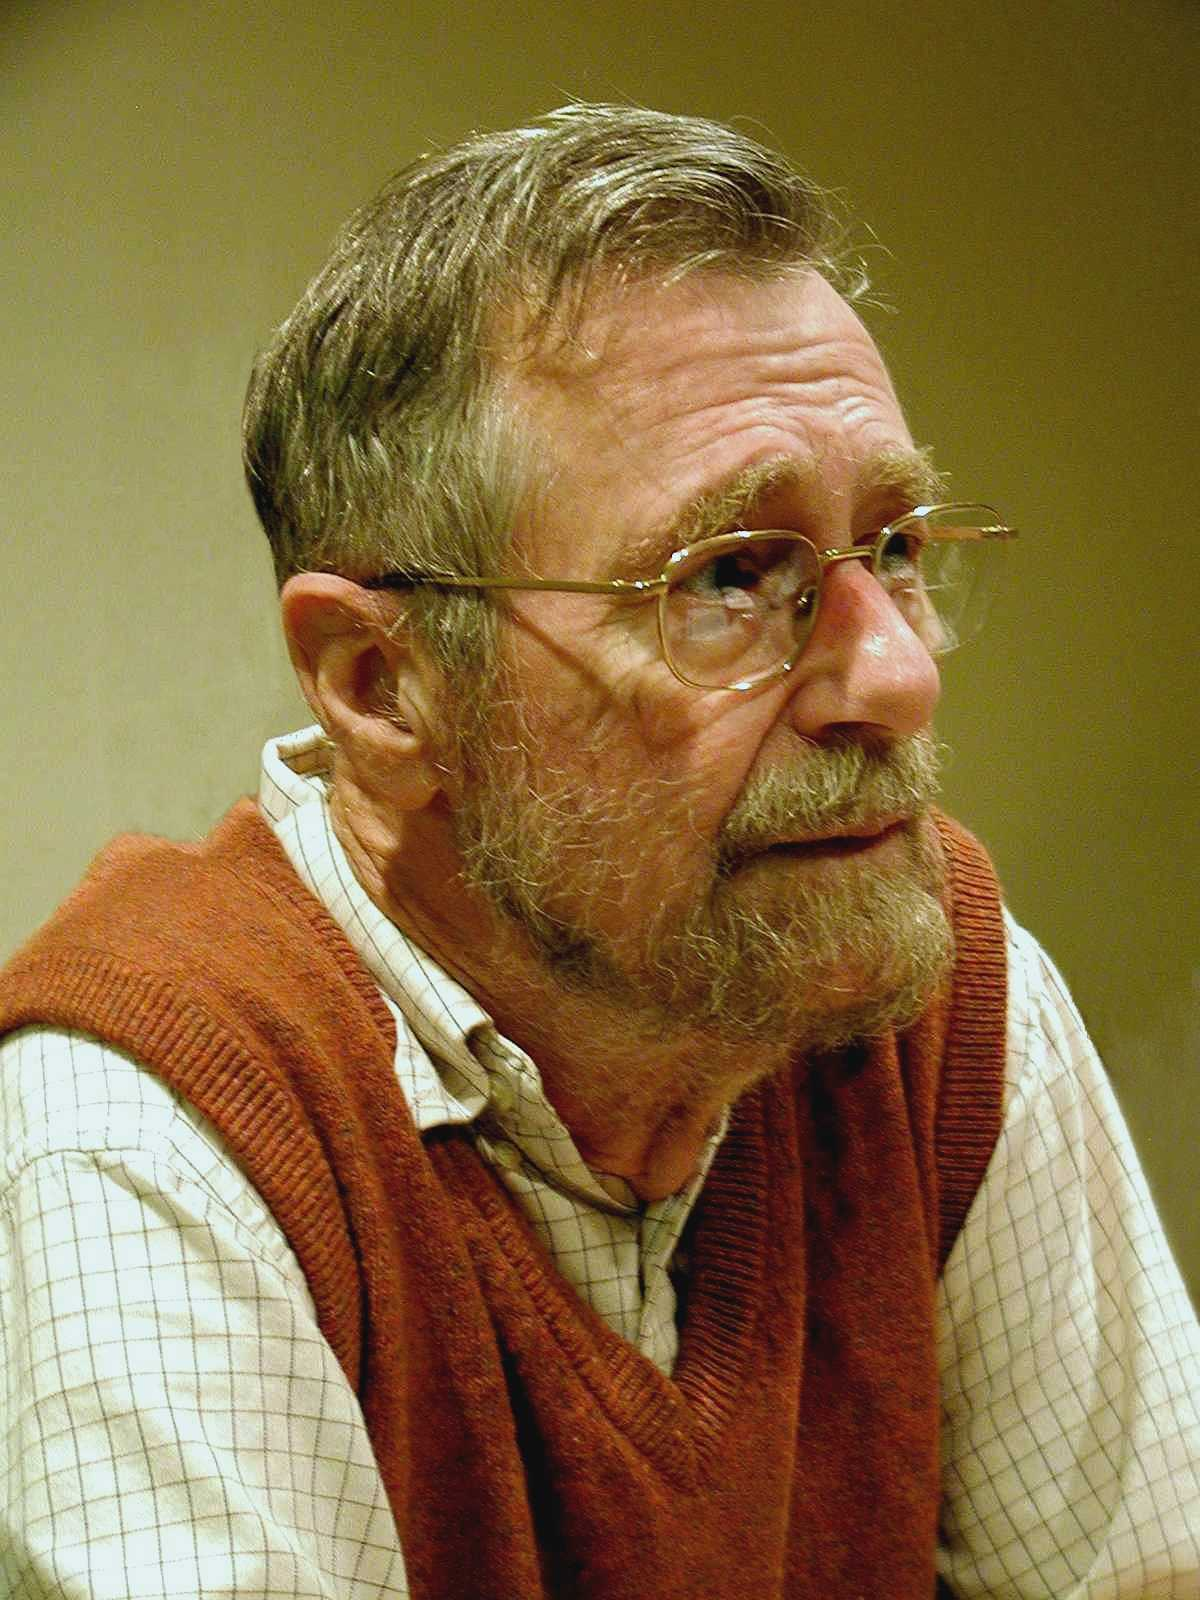
\includegraphics[scale = 0.1]{Djikstra.jpg}
\centering
\caption{\textit{Edgar Djikstra}}
\end{figure}

\begin{small}

 Várias modificações foram sugeridas ao algortimo de Djikstra usando heurísticas para reduzir o tempo de computação exigido na procura do caminho mais curto. Uma das "heurísticas" mais usadas é o \textbf{A*} (aStar) \textit{search algorithm} cujo objectivo é reduzir o tempo de execução reduzindo o espaço de procura. O algortimo A* foi desenvolvido por \textit{Peter Hart} e é uma extensão do algortimo de Djikstra, 1959. 
 
 A algortimo de Djikstra e A* são conceitos muito importantes que queremos reter ao longo do relatório visto que são dos dois algortimos óptimos e que trariam os melhores resultados para o nosso problema. 
 
 Porém, ao longo dos anos novas soluções foram apresentados e em 2009 a google usou um método designado \textit{Contraction hierarchies} que consiste numa técnica que acelera o \textit{shortest path routing} criando um pre processamento do grafo original originando multi camadas de nós organizados hierarquicamente. Desde então o número de algoritmos têm proliferado e hoje em dia somos capazes de encontrar os mais variados algoritmos com tempos de computação espantosos. \textit{Contracted Hierarchies} pode ser usado para encontrar \textit{shortest path routes} de uma maneira muito mais eficiente que o Djikstra e é usado em várias técnicas de \textit{routing} avançadas. Apesar da Google não desvendar que algoritmos usa para estruturar os seus mapas é consensual que será alguma variância de Contracted Hierarchies. \\*
 \end{small}

 
 
\textbf{Hub Labeling Algorithms}


\begin{small}

\textit{Hub labeling} é uma estutura de dados usada para encontrar a distância entre dois pontos num grafo. Providencia um excelente \textit{query time} para \textit{real-world graphs} como redes de estrada e redes sociais. Hub labelling tem dois estados - \textbf{préprocessamento} e \textit{\textbf{querying}}. Enquanto que a parte de \textit{query} é simples o préprocessamento pode demorar muito tempo. Existe um algoritmo para encontrar $O (\log n)$-aproximadamente \textit{Hub Labels} óptimos. No entanto, é lento. A ideia é que os algoritmos de \textit{Hub Labeling} criem uma estratificação hierárquica. Sendo assim os \textbf{HHL} (Hirarchichal Hub Labeling) ordenam os vértices e encontrarm os hub labels que respeitem a ordem. 
Concluindo, os algoritmos de \textit{path finding} têm ganho um grande relevo nos últimos anos e é cada vez mais um assunto a ser investigado e explorado. Apesar do algortimo conseguir resolver os problemas em quase tempo linear, aplicações que abrangem continentes necessitam de algoritmos mais rápidos. O pré processamento torna possivel a exitência de algoritmos sub lineares.
\end{small}

\section{EASY PILOT}
\begin{small}
Após uma introdução ao tema que se vai tratar ao longo do relatório, damos agora uma maior especificação do que vai consistir o nosso projecto. Neste trabalho, pretende-se implementar um navegador que identifique o caminho a seguir, numa dada rede, a partir de uma origem até ao destino desejado. O itinerário poderá ser simples, ou ainda incluir vários pontos de interesse (POIs), como bombas de combustível para reabastecimento, monumentos, ou outros cuja posição sejam indicadas pelo utilizador; outros critérios a utilizar poderão incluir menor distância, menor tempo de viagem, e ainda a existência ou não de pontos de portagem. 
\end{small}

\begin{figure}[H]
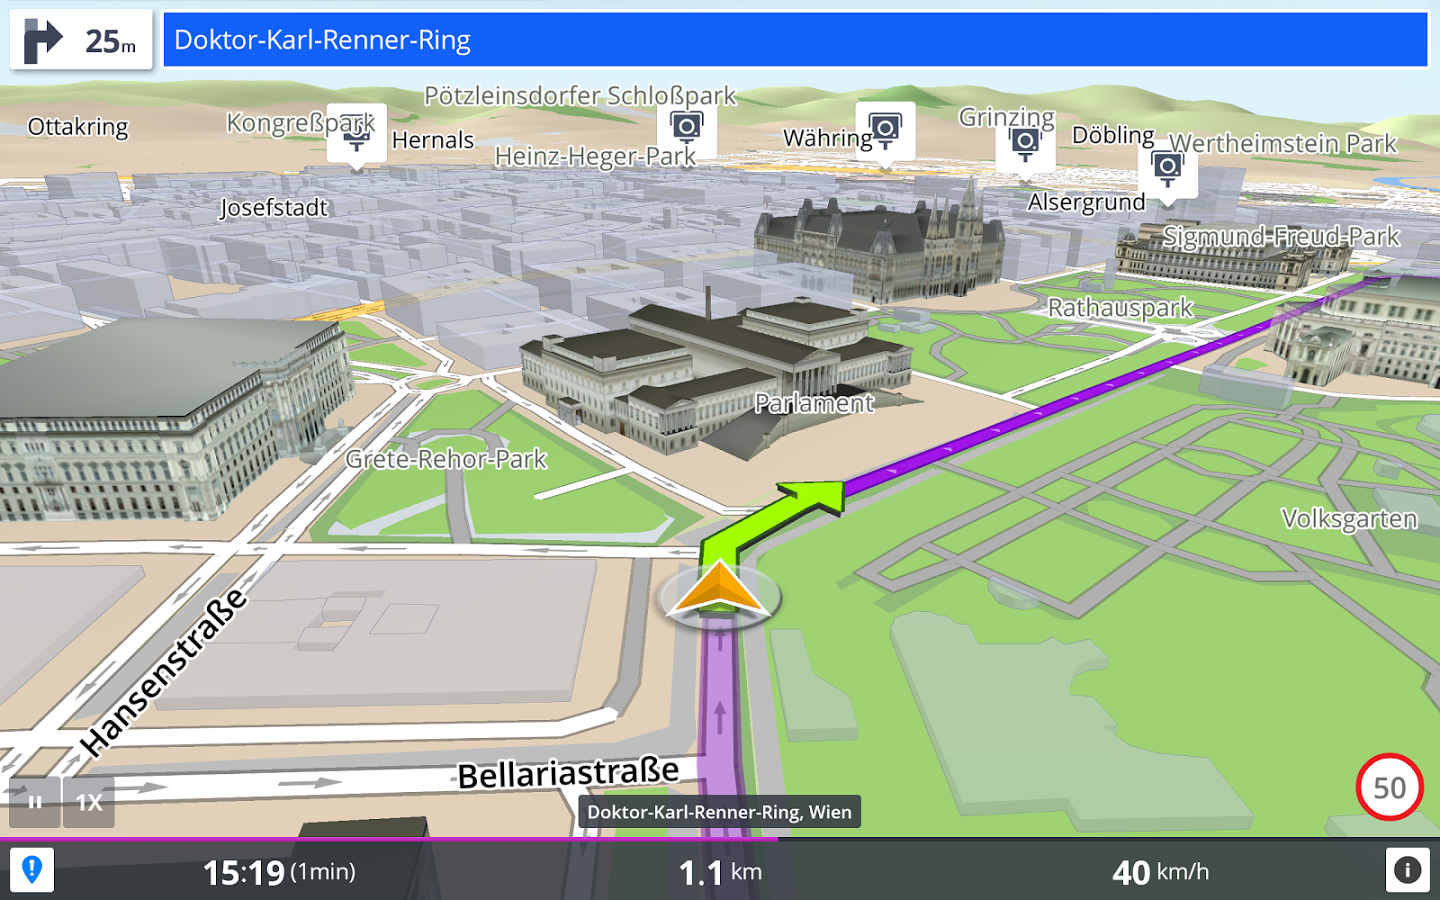
\includegraphics[scale = 0.15]{./GPS.png}
\centering
\caption{Exemplo de um sistema navagação GPS}
\end{figure}


\begin{small}

Para resolver este problema o grupo começou por fazer uma engenharia de requisitos, funcionais e não funcionais e estabelecer metas que acharia pertinentes e exequíveis.

Começamos por decidir qual seria o tamanho mais adequado ao nosso mapa. O mapa teria de ser suficientemente grande para testar várias computações com tempos de execução diferentes mas não poderia ser demasiado grande para que a validação e verificação do software fosse feita de uma maneira mais pragmática. Posto isto, decidimos abranger grande parte da zona do Porto, incluindo a Faculdade de Engenharia da Universidade Do Porto e a Baixa. 

Escolhida a nossa base de dados era necessário ter um \textit{parser} que nos permitisse extrair todas as informações necessárias para formar o nosso \textbf{grafo}. Ao longo das aulas práticas foi-nos informado que essa informação seria facultada pelos monitores da cadeira, mas como tal demorou a acontecer o grupo investigou e conseguiu extrair os seus dados através de outras ferramentas. Para isso utilizadmos um \textit{routing engine} que faz o \textit{parsing} da informação existente no \textit{Open Street Maps} e faz com que seja possível fazer a \textit{route} de toda essa informação. Gera o \textit{SQL Insert scripts} para \textit{PostGIS} compatível com \textit{pgRouting} e \textit{Quantum GIS}. Dada a base de dados, foi feita uma query para gerar a informação que acharíamos pertinente. \\*

\end{small}

\begin{lstlisting}[
           language=SQL,
           showspaces=false,
           numbers=left,
           numberstyle=\tiny,
           showstringspaces=false,
           basicstyle=\ttfamily,
           belowskip=2.0 \baselineskip,
           commentstyle=\color{gray},
           breaklines=true]
    create table vertices as 
    select source as ID, st_makepoint(x1,y1) as geom from edges_table
    union
    select target as ID, st_makepoint(x2,y2) as geom from edges_table
    
    
\end{lstlisting}

Resposta à \textit{query}:

\begin{lstlisting}[
           language=SQL,
           showspaces=false,
           numbers=left,
           numberstyle=\tiny,
           showstringspaces=false,
           belowskip=2.0 \baselineskip,
           basicstyle=\ttfamily\footnotesize,
           commentstyle=\color{gray},
           breaklines=true]
220;"Rua de Sendim";8629;45558;0.0304899;60;-8.6757897;41.1871374;-8.675474;41.1872743
        \end{lstlisting}
        


\begin{small}
Que representam, respectivamente, o \textbf{id}, o \textbf{nome}, o \textbf{source}, \textbf{target}, a \textbf{distancia}, \textbf{a velocidade} \textbf{coordenada X1}, \textbf{coordenada Y1}, \textbf{coordenada X2} e a \textbf{coordenada Y2}.

Nesta tabela cada registo repressenta uma \textbf{aresta}. Cada aresta tem dois \textbf{vértices} \textit{source} e \textit{target} cujas coordenadas estão nas colunas \textit{x1}, \textit{y1}, \textit{x2}, \textit{y2}.

Com esta informação criamos um ficheiro de texto (.txt) que mais tarde seria utilizada para preencher o nosso grafo. 
\end{small} \\


\section{Q \& A}

\newcommand\Que[1]{%
   \leavevmode\par
   \stepcounter{question}
   \noindent
   \thequestion. Q --- #1\par}

\newcommand\Ans[2][]{%
    \leavevmode\par\noindent
   {\leftskip37pt
    A --- \textbf{#1}#2\par}}

\Que{Como vai ser representado o mapa?}
\Ans{Vai ser representado através de um grafo dirigido}

\Que{Quais serão os elementos do grafo?}
\Ans{\begin{itemize}
    \item Vértices (\textit{vertexes}) que têm uma informacao, que e um comparável, neste caso uma \textit{intersection}.
    \item Arestas (\textit{Edges}) que representam as ruas. 
    \item Um Estado inicial que será o sítio de onde o utilizador se quer deslocar
    \item Um Estado Final que será o local para onde o utilizador quer ir. 
    \item Todos os vértices devem ser atingíveis.
\end{itemize}}

\Que{O que é um caminho ponta a ponta e o que é que representa?}
\Ans{É um caminho que começa num local e acaba noutro, neste caso representa a viagem que o utilizador quer realizar.}

\Que{Como é dado o comprimento de um caminho?}
\Ans{O comprimento do caminho é dado através do somatório total do comprimento das arestas}

\Que{Quais foram os algoritmos utilizados para resolver o problema?}
\Ans{\textbf{Djikstra} e \textbf{A*}(A star) foram os algoritmos utilizados para chegar a uma solução óptima do problema.\linebreak\linebreak\linebreak}



\section{FORMALIZAÇÃO DO PROBLEMA}

\begin{small}
Formalizamos agora o problema de acordo com aquela que achamos ser a melhor forma para resolver aquilo a que nos propusemos. \\*
\end{small}

\begin{itemize}
    \item \textbf{\Large{Input}}. \\*
    $ G < V, E > $
    V: Pontos do mapa \\*
    E: Ligação entre dois pontos - ruas. \\*
    \item \textbf{\Large{Output}}. 
    
    Path = $V_{i},I$ = $1...n$ \\*
    Value \\*

    \item \textbf{\Large{Objectivo}}
    
    $\min(valor)$

    $valor$ = $\sum_{i=1}^{n} E_{ij}$\\*
    
    
    \item \textbf{\Large{Restrição}}
    
    $\forall {i} \in Path = \{V_{i}\}$
    
    $\exists {j} \in  Path : V_{i} = V_{j} \wedge i \neq j$\\*
    
    \end{itemize}
    
\setcounter{secnumdepth}{0}
\section{ASSUMPÇÕES DO PROBLEMA}

\begin{itemize}
    \item Dado que tivemos que encurtar o grafo para que fosse mais fácil para efeitos de validação, nem todos os \textbf{vértices} têm solução. Porém,  aplicada uma verificação para saber se é possível e se não é requistado que o utilizador introduza novos valores.
    
    \item A route será calculada será sempre a mais óptima e eficiente consoante o algoritmo escolhido.
\end{itemize}

\setcounter{secnumdepth}{0}
\section{SOLUÇÃO CONCEPTUAL}

\subsection{Djikstra}


Para encontrar uma solução, um dos algoritmos que implementamos foi o \textbf{Djikstra} que já foi falado ao longo do relatório. Decidimos usar o Djikstra porque este permite encontrar o \textbf{caminho mais curto} entre dois pontos considerando apenas o seu custo real. \\


\textbf{Tempo computacional do Djikstra:}\\

 $O\left ( \left | E \right | + \left | V \right |  \log \left | V \right | \right ))$\\

Dijkstra tem uma função de um custo que é o valor real da \textit{source} para o \textit{target}. \\

 $f(x) = g(x)$ \\


Dijkstra não tem heurística e a cada passo escolhe arestas com o custo inferior, ou seja, tende sempre a cobrir uma área muito maior do nosso grafo. 

Este algoritmo é um algoritmo ganancioso, tomando decisões que parecem óptimas no momento, determinando assim o conjunto de melhores caminhos intermediários. \\*



\subsection{Pseudo código}

\begin{enumerate}
    \item Inicialização de todos os nodes com distância "infinita"; inicialização da starting node a 0;
    \item Marcar a distância da starting node como permanente e todas as outras como temporárias
    \item Marcar a \textit{starting node} como activa;
    \item Calcular as distâncias temporárias de todos os vértices vizinhos do vértice \textit{activo} somando a sua distância com o peso das arestas;
    \item Se a distância calculada de um vértice for inferior ao que está a ser examinado, fazer \textit{update} à distância e colocar o vértice activo como antecessor. Este é um processo de \textit{update} e é fundamental no funcionamento do Dijkstra.
    \item Colodar o vértice com a menor distância temporária como activo e marcar a sua distância como permanente. 
    \item Repetir os passos 4 a 7 até não existirem mais vértices com distância permanente cujos vizinhos tenham distâncias temporárias. 
\end{enumerate}


\begin{lstlisting}[
           language=C++,
           showspaces=false,
           numbers=left,
           numberstyle=\tiny,
           showstringspaces=false,
           basicstyle=\ttfamily\footnotesize,
           commentstyle=\color{gray},
           breaklines=true,
           belowskip=3.0 \baselineskip
        ]
        function Dijkstra(Graph, source):
        for each vertex v in Graph: 	// Inicializacao
        dist[v] := infinity 	// distancia inicial da source ate ao vertex v posta infinito
 	previous[v] := undefined 	// Previous node in optimal path from source
 	dist[source] := 0 	// Distancia da source a source
 	Q := the set of all nodes in Graph 	// todos os nos no grafo nao foram processatos e sao adicionados a Q (pode ser priority queue)
 	while Q is not empty: 	// main loop
 	u := node in Q with smallest dist[ ]
 	remove u from Q
 	for each neighbor v of u: 	// v nao foi removido de Q 
 	alt := dist[u] + dist_between(u, v)
 	if alt < dist[v] 	// Relax (u,v)
 	dist[v] := alt
 	previous[v] := u
 	return previous[ ] 

\end{lstlisting}



\subsection{Implementação}


Esta foi a implementação do grupo:


\begin{lstlisting}[
           language=C++,
           showspaces=false,
           showstringspaces=false,
           numbers=left,
           numberstyle=\tiny,
           basicstyle=\ttfamily\footnotesize,
           commentstyle=\color{gray},
           breaklines=true,
           belowskip=3.0 \baselineskip
        ]
        
        template<class T>
void Graph<T>::DijkstraShortestPath(const T &start){		//baseado teorica 06.grafos2_a

	for(unsigned i=0; i<getNumVertex(); i++){
		vertexSet[i]->path = NULL;
		vertexSet[i]->setDistance(INF);
		vertexSet[i]->processing = false;
	}

	Vertex<T> *s = vertexSet[addVertex(start)];
	s->setDistance(0);

	vector<Vertex<T>*> pq;

	pq.push_back(s);

	make_heap(pq.begin(), pq.end());

	while(!pq.empty()){

		s = pq.front(); // diferente do git daquele gaj
		pop_heap(pq.begin(), pq.end());
		pq.pop_back();

		for(unsigned i=0; i<s->adj.size(); i++){

			Vertex<T> *w = s->adj[i].dest;

			if( (s->distance + s->adj[i].length) < w->distance){

				w->setDistance(s->distance + s->adj[i].length);
				w->path = s;

				if(!w->processing){
					w->processing = true;
					pq.push_back(w);
				}

				make_heap(pq.begin(), pq.end(), vertex_greater_than<T>());
			}
		}
	}

}
        
       
\end{lstlisting}


\subsection{Resultados}

Dado que o Dijkstra tem em atenção o tamanho do grafo para realizar a sua computação, realizamos vários testes nos quais aumentamos a nossa base de dados. Como dito anteriormente, a nossa base de dados original tinha informação de todo o distrito do Porto. Com vista a avaliar os resultados e compreender se estão de acordo com com o esperado e aquilo que é o funcionamento do Dijkstra. 

\begin{figure}[H]
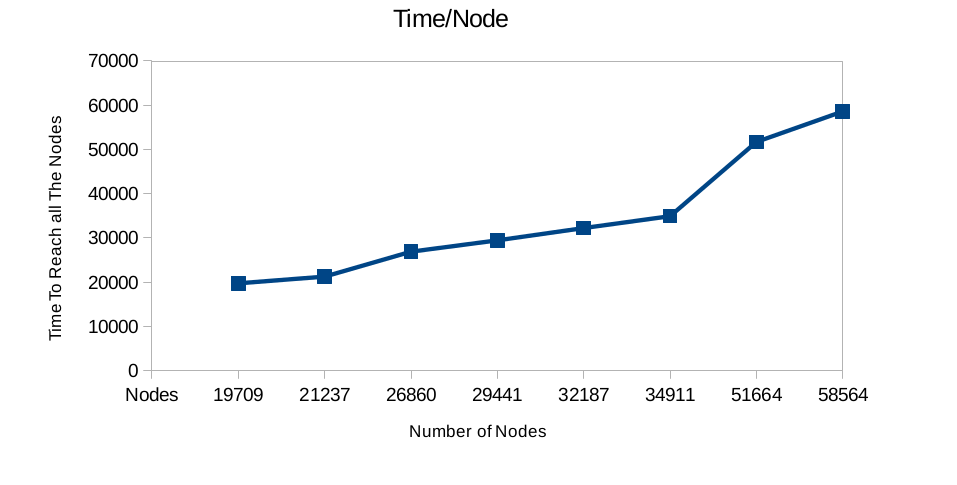
\includegraphics[scale = 0.5]{./Djikstra_Graph.png}
\centering
\caption{Grárfico tempo de computação Djikstra por número de nodes}
\end{figure}

Tal como previamos a função do djikstra ao longo do tempo tem uma evolução logaritmica. Apesar de não ser bem compreensível através da imagem, se tivessemos colocado mais pontos, ou seja, uma maior variedade do número de vértices o Djikstra iria demorar mais tempo a executar. Isto acontece porque Djikstra não possui heurísticas, ou seja, quanto maior for o grafo maior serão o número de vértices e consequentemente o tempo que o algoritmo vai demorar a chegar a todos os vértices pelo seu \textit{real cost} também será maior. 



\begin{table}[h]
\centering
\begin{tabular}{ll}
Time(s)      & Nodes \\
0.2076189965 & 1979  \\
0.2234530002 & 21237 \\
0.2633250058 & 26860 \\
0.2849009931 & 29441 \\
0.3500050008 & 32187 \\
0.4250009954 & 34911 \\
0.9803569913 & 51664 \\
0.9691500068 & 58564
\end{tabular}
\caption{Tabela de Resultados}
\label{my-label}
\end{table}

\setcounter{secnumdepth}{0}
\section{UMA SOLUÇÃO MELHORADA}

\subsection{A*} 


Como esforço complementar e por questões de compreensão e brio, o grupo decidiu implementar um segundo algoritmo, o \textbf{A*}. O A* foi um algoritmo que foi descrito pela primeira vez em 1968 por Peter Hart, Nils Nilsson e Bertram do \textit{Instituto de pesquisa de Stanford}. \textbf{A*} é uma variação ou generalização do \textbf{Djikstra} sendo que a sua principal diferença é que o \textbf{Djikstra} não usa heurísticas para encontrar a melhor aproximação ao caminho mais curto.

Porém, muitas vezes surgem más interpretações em relação a estes dois algoritmos pelo que tentamos esclarecer alguns conceitos.\\

\textit{O A* é mais rápido que o Djikstra e usa uma best-first-search para acelerar o processo.}

O \textbf{A*} é uma variação do Djikstra. A* é considerado um \textit{best-first-search} porque gananciosamente escolhe qual o vértice a explorar de seguida de acordo com o valor de \\*

$g(x) = h(x) + g(x)$\\*


onde o \textit{h} é a \textbf{heurística} e o g o custo até ao momento. 


Notar que se se usar uma heurística não informativa, $h(x) = 0$ para cada vértice, faz-se com que o \textbf{A*} escolha o vértice a desenvolver baseado no "custo até ao momento", o mesmo que o algoritmo de Djikstra. Portanto, se $h(x) = 0$, \textbf{A*} volta a ser \textbf{Djikstra}. \\


\textit{Se eu precisar de um algoritmo para correr em milissegundos, quando é que o \textbf{A*} se torna mais promissor?}

Não é algo que seja linear e depende de alguns conceitos. Se tiver uma heurística decente (\textit{e.g Greedy best first}) é mais rápido que o \textbf{A*} mas não é, de todo, uma solução óptima. \\

\textit{A* não retorna necessariamente os melhores resultados}


A* é completo (encontra um caminho se existir) e óptimo (encontra sempre o \textbf{caminho mais curto}) se usarmos uma função heurística admissível. \\


\textit{Se precisar de resultados rápidos, é melhor pré-computar os caminhos? Pode ocupar megabytes de espaço para os guardar}


Em alguns problemas, pré computar é uma optimização coumum como por exemplo no problema \textit{15-puzzle}, mas muito mais avançada. O caminho de um ponto A para um ponto B é chamado um \textbf{macro}. Alguns caminhos são muito úteis e devem ser relembrados. \textbf{Machine learning} é adicionado ao algoritmo de maneira que os Macros possam ser memorizados mais facilmente.\\

Resumindo, \textbf{A*} apenas expande um vértice se este parecer promissor. Apenas se foca em atingir o vértice final do vértice actual e não todos os outros vértices. É óptimo, se a heurística for admissível. Então, se a heurística é boa para aparoximar o custo futuro, vão ser precisos serem examinados muito menos vértices que com o \textbf{algoritmo de Djikstra.}

\subsection{Pseudo código}

\begin{lstlisting}[
           language=C++,
           showspaces=false,
           numbers=left,
           numberstyle=\tiny,
           showstringspaces=false,
           basicstyle=\ttfamily\footnotesize,
           commentstyle=\color{gray},
           breaklines=true,
           belowskip=3.0 \baselineskip
        ]
function A*(start, goal)
    // The set of nodes already evaluated.
    closedSet := {}
    // The set of currently discovered nodes still to be evaluated.
    // Initially, only the start node is known.
    openSet := {start}
    // For each node, which node it can most efficiently be reached from.
    // If a node can be reached from many nodes, cameFrom will eventually contain the
    // most efficient previous step.
    cameFrom := the empty map

    // For each node, the cost of getting from the start node to that node.
    gScore := map with default value of Infinity
    // The cost of going from start to start is zero.
    gScore[start] := 0 
    // For each node, the total cost of getting from the start node to the goal
    // by passing by that node. That value is partly known, partly heuristic.
    fScore := map with default value of Infinity
    // For the first node, that value is completely heuristic.
    fScore[start] := heuristic_cost_estimate(start, goal)

    while openSet is not empty
        current := the node in openSet having the lowest fScore[] value
        if current = goal
            return reconstruct_path(cameFrom, current)

        openSet.Remove(current)
        closedSet.Add(current)
        for each neighbor of current
            if neighbor in closedSet
                continue		// Ignore the neighbor which is already evaluated.
            // The distance from start to a neighbor
            tentative_gScore := gScore[current] + dist_between(current, neighbor)
            if neighbor not in openSet	// Discover a new node
                openSet.Add(neighbor)
            else if tentative_gScore >= gScore[neighbor]
                continue		// This is not a better path.

            // This path is the best until now. Record it!
            cameFrom[neighbor] := current
            gScore[neighbor] := tentative_gScore
            fScore[neighbor] := gScore[neighbor] + heuristic_cost_estimate(neighbor, goal)

    return failure

function reconstruct_path(cameFrom, current)
    total_path := [current]
    while current in cameFrom.Keys:
        current := cameFrom[current]
        total_path.append(current)
    return total_path     
       
\end{lstlisting}

\subsection{Implementação}

\begin{lstlisting}[
           language=C++,
           showspaces=false,
           numbers=left,
           numberstyle=\tiny,
           showstringspaces=false,
           basicstyle=\ttfamily\footnotesize,
           commentstyle=\color{gray},
           breaklines=true,
           belowskip=3.0 \baselineskip
        ]
        
template <class T>
float heuristic_aStar(Vertex<T> *s, Vertex<T> *t, bool dt){
	return (sqrt(pow(s->getIntersection().getCoord().x - t->getIntersection().getCoord().x, 2) + pow(s->getIntersection().getCoord().y - t->getIntersection().getCoord().y, 2)));
}


template<class T>
void Graph<T>::updateFlood(Vertex<T>* vertex, T goal) {
	if((vertex->closed != NULL) && (!(vertex->closed)))
		return;

	for(int i = 0; i < vertex->adj.size(); i++) {

		vertex->adj[i].getDest()->setDistance(vertex->adj[i].getDest()->getDistance()  + vertex->adj[i].getLength());
		vertex->adj[i].getDest()->fx = vertex->adj[i].getDest()->getDistance() + heuristic_aStar(vertex, vertexSet[addVertex(goal)],1);
		updateFlood(vertex->adj[i].getDest(), goal);

	}
}

template <class T>
void Graph<T>::aStar(const T &start, const T &goal, bool dist){ //MAKE THIS BOOL

	for(unsigned i = 0; i < vertexSet.size(); i++) {
		vertexSet[i]->path = NULL;
		vertexSet[i]->distance = INF;
		vertexSet[i]->fx = INF;
		vertexSet[i]->closed = NULL;
		vertexSet[i]->inQueue = false;
	}


	Vertex<T> *s = vertexSet[addVertex(start)];

	s->setDistance(0);
	s->closed = false;
	s->fx = s->getDistance() + heuristic_aStar(s, vertexSet[addVertex(goal)], dist);

	vector<Vertex<T>*> pq;		//nextVertices

	pq.push_back(s);
	s->inQueue = true;

	//cout << s->getIntersection().getID() << endl;

	make_heap(pq.begin(), pq.end());

	while (!pq.empty()) {
		Vertex<T> *current = pq.front();
		pop_heap(pq.begin(), pq.end());
		pq.pop_back();


		current->inQueue = false; //extra(?)

		if (current == vertexSet[addVertex(goal)])
			break;


		current->closed = true;

		for(unsigned i = 0; i < current->adj.size(); i++) {
			Edge<T> edge = current->adj[i];
			Vertex<T> *neighbour = edge.dest;
			double weight = dist ? edge.length : neighbour->time;

			if(neighbour->closed == NULL) {
				neighbour->closed = false;
				neighbour->distance = current->distance + weight;
				neighbour->path = current;
				neighbour->fx = neighbour->distance + heuristic_aStar(neighbour, vertexSet[addVertex(goal)], dist);

				pq.push_back(vertexSet[addVertex(neighbour->getIntersection())]);

			}

			if (!neighbour->closed) {
				if (neighbour->distance > current->distance + weight) {
					neighbour->distance = current->distance + weight;
					neighbour->path = current;
					neighbour->fx = neighbour->distance + heuristic_aStar(neighbour, vertexSet[addVertex(goal)], dist);
				}
			}


			if(neighbour->closed) {
				if(neighbour->distance > current->distance + weight) {
					neighbour->path = current;
					neighbour->distance = current->distance + weight;
					neighbour->fx = neighbour->distance + heuristic_aStar(neighbour, vertexSet[addVertex(goal)], dist);
					updateFlood(neighbour, goal); //com problemas
				}
			}

			make_heap(pq.begin(), pq.end(), vertex_greater_than_fx<T>());

		}
	}


	return;
}

\end{lstlisting}


\subsection{Heurística}

A função heurística $h(n)$ diz a \textbf{A*} uma estimativa do custo mínimo de cada vértice(source) até outro(target). É muito importante escolher uma boa função heurística. 

A heurística pode ser usada para controlar o comportamento do \textbf{A*}.

\begin{itemize}
    \item Num extremo se $h(n)$ é 0, então apenas o $g(n)$ tem preponderância e o A* transforma-se no algoritmo de Djikstra e é garantido que vai encontrar \textbf{o caminho mais curto.}
    \item Se o $h(n)$ é sempre \textbf{menor (ou igual)} ao custo de mover de $n$ até ao \textit{goal}, então A* é garantido que encontra o \textbf{caminho mais curto}. Quando menor for $h(n)$, mais o A* se expande, fazendo com que seja \textbf{mais lento.}
    \item Se $h(n)$ for \textbf{exactamente igual} ao custo de se mover de $n$ até ao \textit{goal}, então A* seguirá \textbf{o melhor caminho} e nunca vai expandir mais nada, o que o torna \textbf{muito rápido}. Apesar de não poder ser possível fazer isto acontecer na maior parte dos casos, é possível faze-lo exacto em alguns casos especiais. É entusiasmante saber que se dermos a informação perfeita, A* comportar-se-á na perfeição também.
    \item Se às vezes o $h(n)$ é maior que o custo de se mover de $n$ para \textit{goal}, então não é garantido que A* possa encontrar o \textbf{caminho mais curto} mas vai ser mais rápido.
    \item No outro extremo, se $h(n)$ é muito alto em relação a $g(n)$, então apenas o $h(n)$ tem preponderância e o A* transforma-se num \textit{Greedy Best-First-Search}.
\end{itemize}

Então temos uma situação interessante em que podemos decidir o que queremos retirar do A*. Num ponto exacto, com a informação perfeita, retiraremos o \textbf{caminho mais curto} de uma maneira rápida. Se estivermos muito abaixo do esperado vamos continuar a ter o caminho mais curto mas de uma maneira lenta. Se estivermos muito acima, não teremos o caminho mais curto, mas o A* terá uma boa \textit{performance}.

Falamos agora de três heurísticas para calcular a distância. Notar que existem muitas mais mas que tivemos estas em contas por estarem associadas ao movimento e serem de simples implementação.

\begin{itemize}
    \item \textbf{Manhattan distance}. Normalmente usada em \textit{square grids} que permitem movimento de 4 direcções. É a heurística \textit{standard}.
    \item \textbf{Diagonal Distance}. Usada em \textit{square grids} que permitem movimento em 8 direcções. Inclui os 4 movimentos tradicionais (cima, baixo, esquerda, direita) mais os movimentos diagonais.
    \item \textbf{Euclidean distance}. Se nos pudermos mover em qualquer direcção, esta é a melhor heurística porque permite calcular uma linha directa de um ponto ao outro.
\end{itemize}

Para o nosso projecto decidimos usar a \textbf{distância Euclideana} visto que no nosso grafo e de um vértice para o outro podemos movimentarmos em mais que uma direção e calcular a distância de um ponto ao outro seria muito mais imediato.


\section{DIAGRAMA DE CASOS DE USO}

\begin{figure}[H]
\vspace*{-1.5cm}
\hspace*{-2.5cm}   
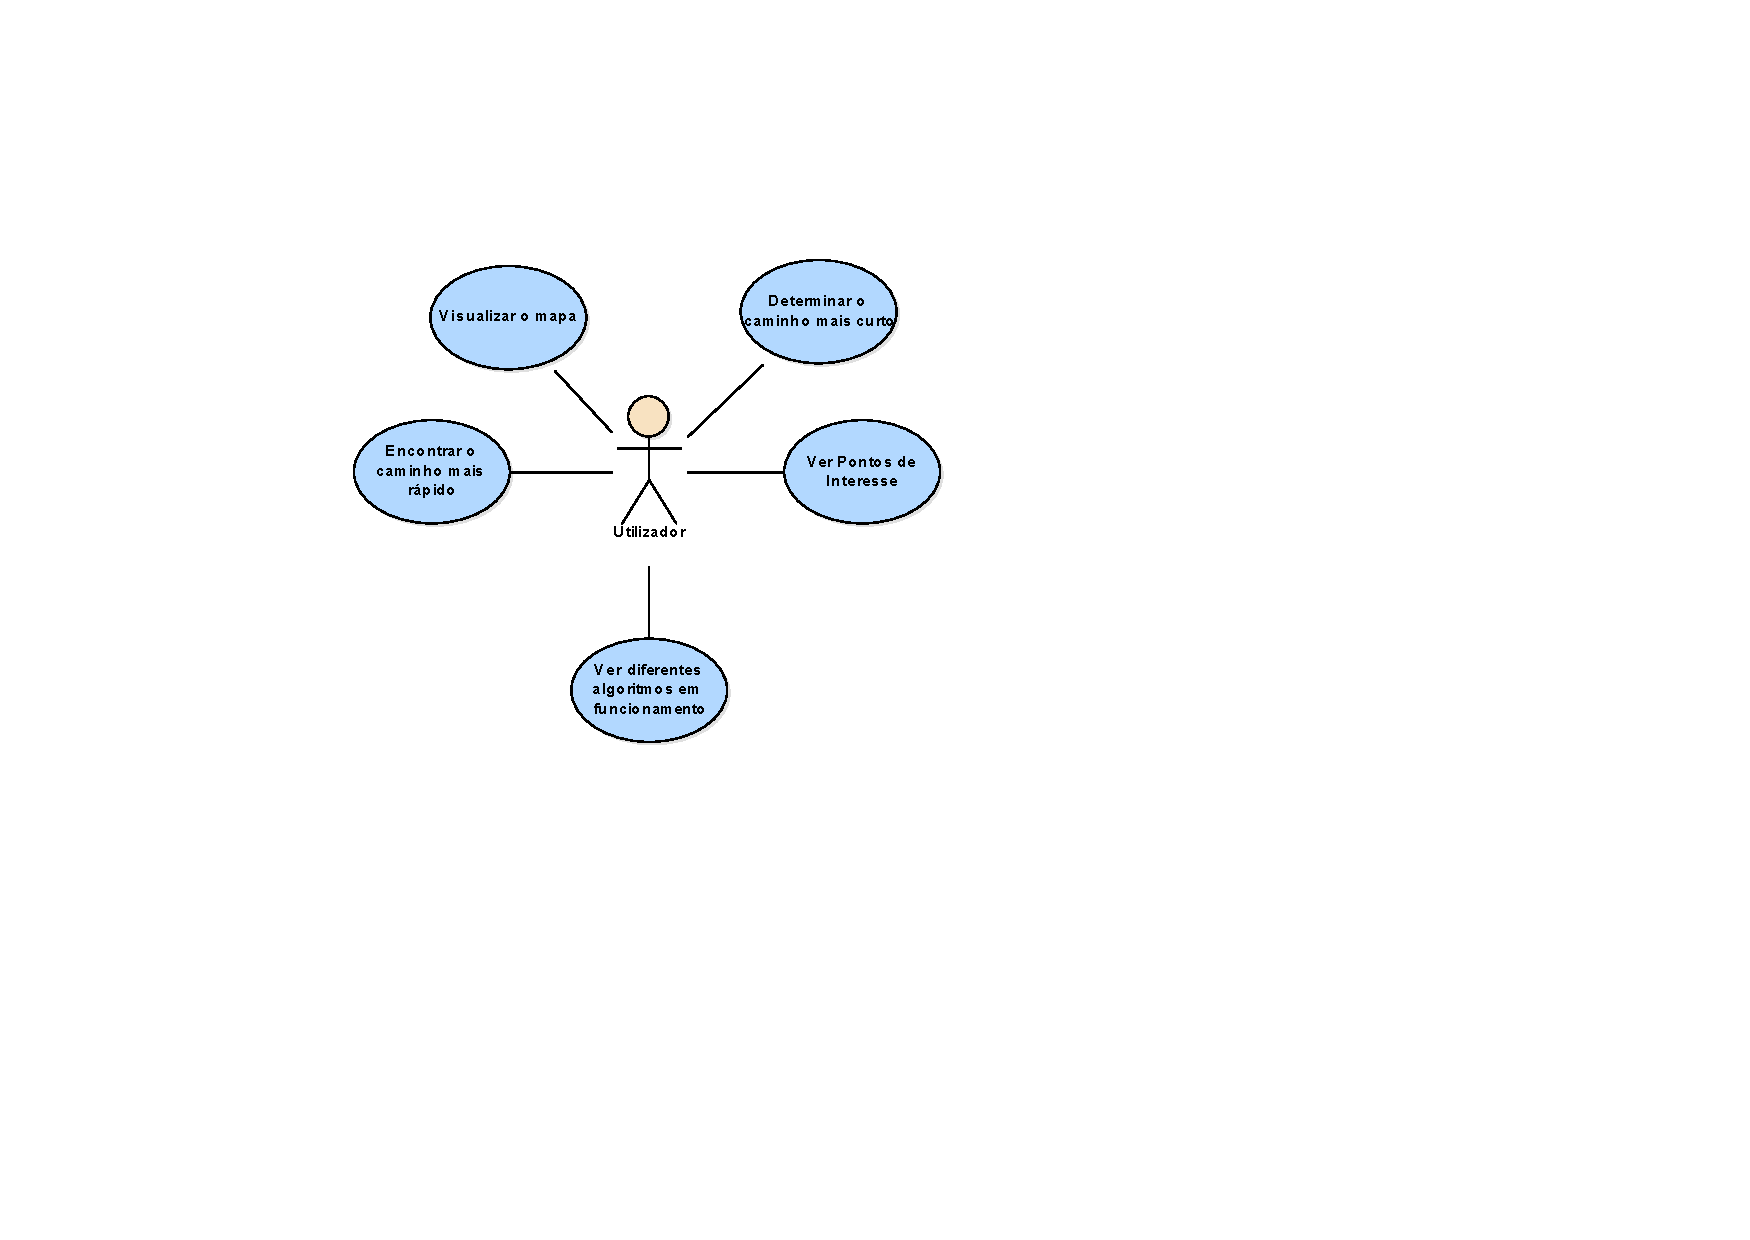
\includegraphics[scale = 1.0]{DiagramaCasoDeUso.pdf}
\centering
\caption{\textit{Diagrama de Casos de Uso}}
\end{figure}

\section{DIAGRAMA DE CLASSES}

\begin{figure}[H]
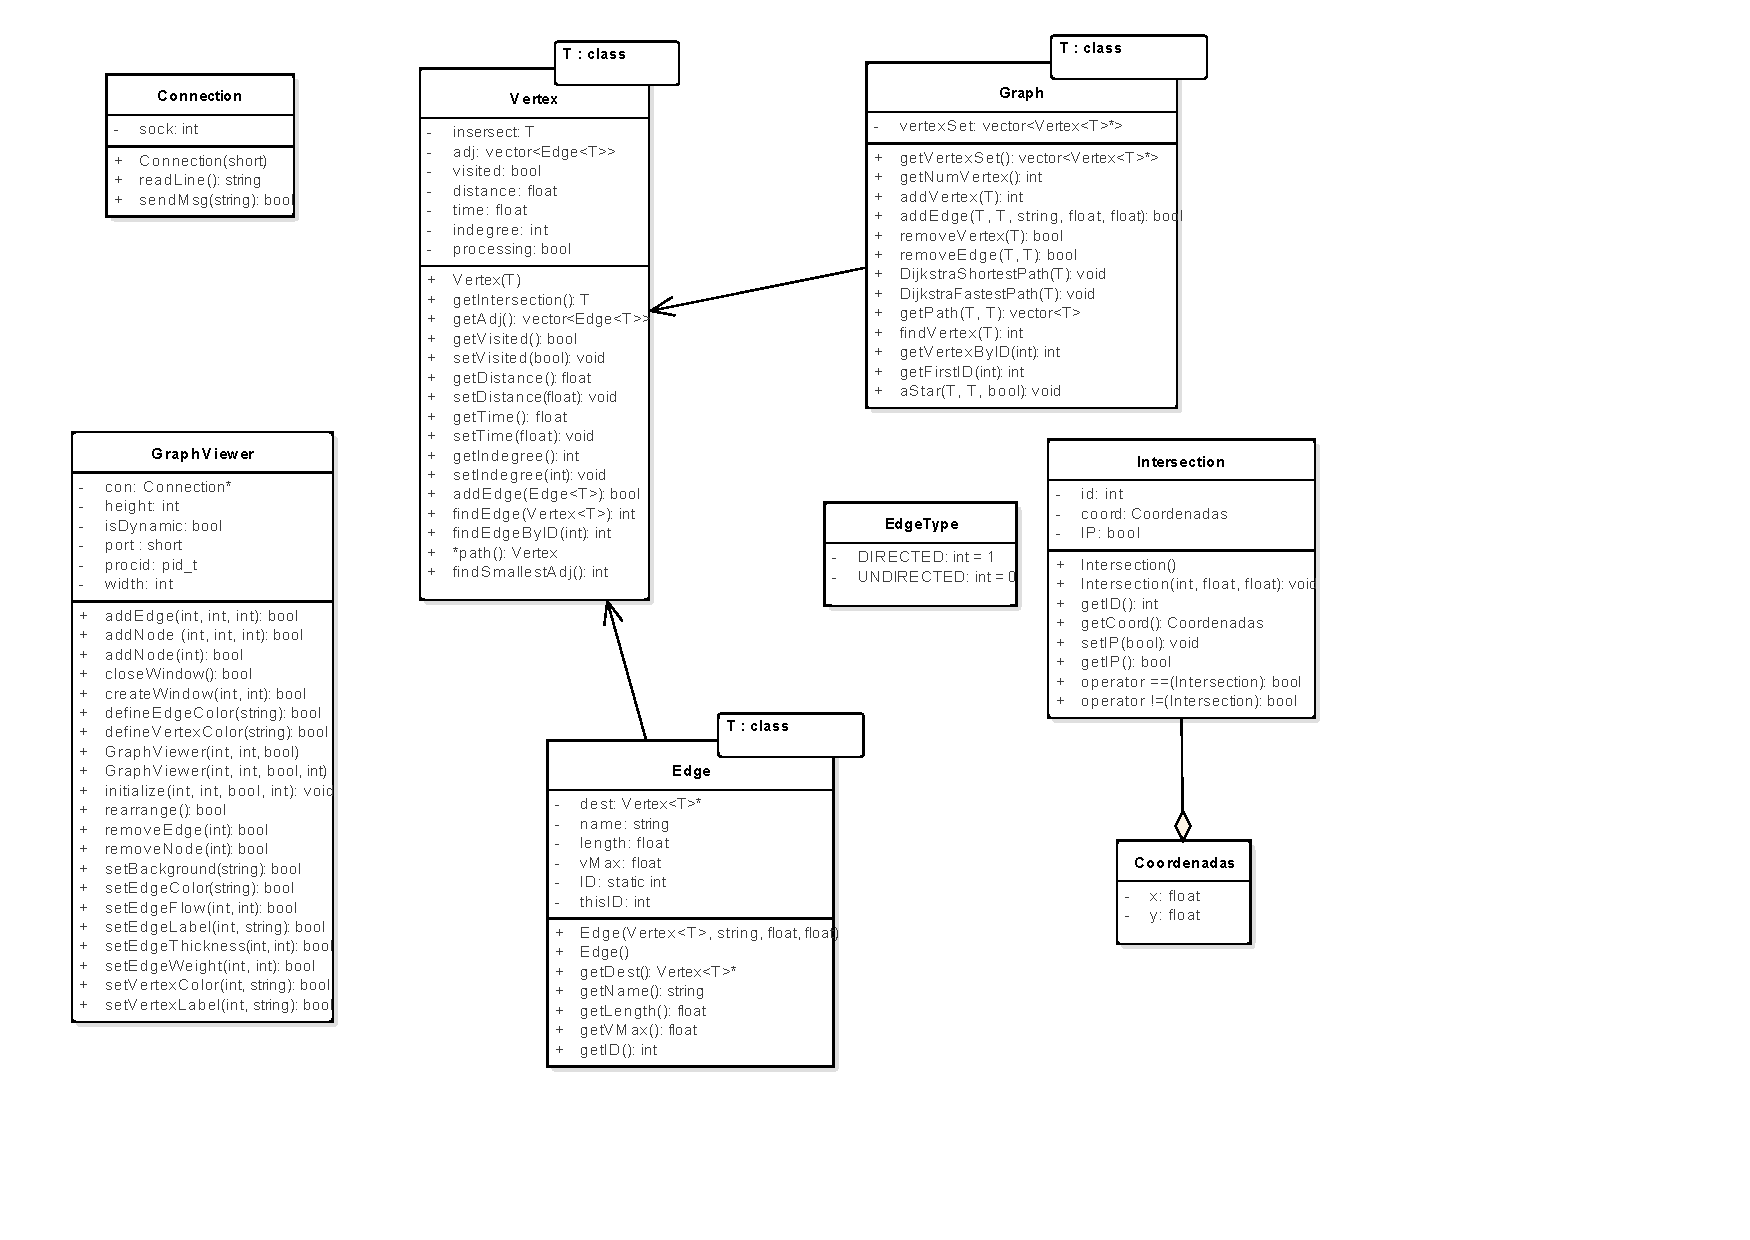
\includegraphics[scale = 0.7]{DiagramaDeClassesCAL}
\centering
\caption{\textit{Diagrama de Classes}}
\end{figure}

\section{CONCLUSÕES E TRABALHO FUTURO}

\begin{small}
Terminado o relatório e após toda a investigação feita deixamos algumas conclusões que achamos ser pertinentes e relatam o percurso e actividades do grupo.

Começamos por enaltecer toda a dedicação do grupo na maneira como encarou este desafio e tentou esmiuçar os conceitos. Desde o ínico que o nosso foco foi tentar aprender o mais possível e tirar conclusões que realmente fosse apalpáveis e com carácter pedagógico. Começando pelo parser que foi conseguido 100\% por trabalho nosso e que nos permitiu começar o trabalho e tratar a informação da maneira mais conveniente. Nesse processo entramos em contacto com ferramentas nunca usadas bem como conhecimentos que não foram adquiridos até ao mesmo momento como o \textit{PostGIS}. 
Numa primeira fase do trabalho, implementamos o algoritmo \textbf{Djikstra} mas achamos que tornaria tudo bastante linear e que os nossos conhecimentos não estavam a ser explorados pelo que partimos para uma nova implementação, de uma solução óptima que nos permitisse comparar resultados e perceber em que casos essas soluções se adequam ou são mais eficientes. 
Temos noção de que o algortimo \textbf{A*} foi bastante trabalhoso e que nos atrasou na entrega e, estando alerta das consequências que atraso pode acarretar, decidimos fazer um último esforço para concretizar aquilo que sempre tivemos planeado.

Tivemos dificuldades na construção da interface. Encontrar uma função que convertesse coordenadas geográficas em pixéis foi algo que nos tomou algum tempo e que não conseguimos encontrar uma solução perfeita. Mesmo usando algumas fórmulas para dimensionar o nosso \textit{background
} (mapa do Porto) ao sítio onde era colocado o nosso grafo, este nunca ficou no sítio e tivemos de o ajudar através de um processo bruteforce, alterando as coordenadas \textit{x} e \textit{y} até estas estarem nos limites do \textit{background}.
Tivemos também algumas dificuldades na implementação do algoritmo A* e apesar de estar ser encontrar uma solução que calcula o \textit{shortest path}, está não está 100\% optimizada e precisaria de alguns ajustes. 

Posto isto, agradecemos a oportunidade que tivemos em fazer um projecto que nos cativou e nos fez ter vontade de saber mais. O grupo dinamizou-se de uma maneira agradável e proactiva sendo que todos os membros se disponibilizaram a mais e melhor e ajuda de cada um foi preciosa.

Para o próximo projecto pretendemos manter a postura e encarar como desafio que pode ser sempre optimizado. 
\end{small}

\section{}

\begin{thebibliography}{9}

\bibitem{lamport94}
  Stack Overflow, \url{http://stackoverflow.com/}

\end{thebibliography}

\end{document}